\documentclass[12pt]{article}
\usepackage[utf8]{inputenc}
\usepackage{amsmath}
\usepackage{graphicx}
\usepackage{xcolor}
\usepackage{listings}
\usepackage{hyperref}
\usepackage{enumitem}
\usepackage{longtable}
\def\_{\textunderscore\-}



\title{Resourceful}
\author{Lucian Carata \and Oliver Chick \and James Snee}
\date{}
\begin{document}
\lstdefinestyle{customc}{
  belowcaptionskip=1\baselineskip,
  frame=lines,
  numbers=left,
  breaklines=false,
  language=C,
  showstringspaces=false,
  basicstyle=\scriptsize\ttfamily,
  keywordstyle=\bfseries\color{green!40!black},
  commentstyle=\color{purple!40!black},
  identifierstyle=\color{blue},
  stringstyle=\color{orange},
}
\maketitle{}

\begin{abstract}
Some applications spend a significant amount of time in the Linux kernel \cite{kernelscale}, but understanding any variation in execution time and other consumed resources (cpu, memory, disk, network) at the level of a system call remains challenging.
Existing methods for resource accounting are either too coarse grained (per-task or system-wide tools like perf, iostats, latencytop) or too fine grained (the FTrace function tracer) incurring significant overheads (3x) and requiring post-processing in user-space.
Furthermore, no attempts have been made to quantify delayed resource consumption generated by a particular system call. Such asynchronous operations are invisible from the perspective of the application, but add to the cost of running it and may affect the performance of other applications running concurrently.
\end{abstract}

\section{Resourceful---high level overview}
  As an answer to the above problems, we propose \emph{Resourceful}, a framework that provides system call resource consumption aggregated per kernel functional unit \cite{kernelmap}. It reports both costs that were incurred synchronously with the system call as well as those incurred during asynchronous actions triggered by the system call, but executed after its completion (for example, the flushing of a kernel buffer to disk, which may occur after the initial system call returned).

Resourceful exposes a user-space library that developers can use to express interest in the resource consumption made by specific system calls. Calls to this library can be made either explicitly by the developer or inserted as part of application instrumentation. 
%The resource accounting then takes place in the linux kernel which is modified to support the required functionality.
The resource accounting then takes place in the Linux Kernel using probes inserted by the  SystemTap tracing framework.


%We believe that the library, together with the changes made to the Linux kernel to support its features, provide the required primitives for implementing more complex use cases:
We believe that the Resourceful library, together with the SystemTap framework, provide the required primitives for implementing more complex use cases:

\subsection{Use cases}
\begin{enumerate}
\item Enforcing fine-grained quotas in running applications. We envision enabling quotas per application operation (in the example of a server application, per request quotas).
\item Tracking per-request resource consumption in a client/server setup and correlating that with variations in measured performance (end-to-end latency)
\item Explaining performance variations in virtualized environments. For example, understanding why performing I/O operations in a Xen virtualised guest is sometimes slow.
\end{enumerate}


\subsection{Contributions}
\begin{itemize}
%\item A low-overhead kernel-level mechanism for measuring per system call resource consumption (cpu, memory, disk, network) in each functional module of the kernel (see the kernel map in \cite{kernelmap} for a list).
\item Accounting for both synchronous and asynchronous resource consumption inside the operating system kernel.
\end{itemize}


\section{System design}
In this section we describe our design for Resourceful, which exposes primitives to user applications that allow them to better account for the resources consumed by the kernel. 
The aim is to provide these primitives with minimal impact on system performance, so that Resourceful can be feasibly used in a production system.

\subsection{User-space library}
\textbf{Developer’s perspective:\\}
The Resourceful library allows programmers to express their interest in the resource consumption of the next system call, with use of the \texttt{acct\_next} function. After the next system call returns, they can inspect a \texttt{call\_cost} data structure and observe the resource costs it incurred synchronously. 
If the system call incurs any asynchronous costs, the kernel will then account these to the same \texttt{call\_cost} data structure. To access those costs reliably, the user has to either call \texttt{wait\_async\_cost} passing the \texttt{call\_cost} structure or register a callback function (a function that will be called when the kernel detects all asynchronous effects of the system call have been accounted for).

When calling \texttt{acct\_next} developers can also specify which components should be accounted for, which allows them to limit the amount of data being collected.
Below we show an example of how this mechanism works.

\vspace{1em}
\lstset{style=customc, captionpos=b}
\begin{lstlisting}[caption=Sample code using the \texttt{rsrcfl} library]
 void on_cost_done(call_cost* cost, void* ctx){
  //callback; read costs and take actions (aggregate, build histograms, etc)
 }

 int main(int argc, char** argv){
   init_resource_acct(); // called on each thread - does some memory allocation
			 // and calls an ioctl setting up resource accounting.
   int filter = SYS | PROC | NET_SOCK; // defines what resources we're
				       // interested in, default: ALL (include
				       // all resources)
   call_cost *cost_o, *cost_w;
   acct_next(&cost_o, filter);         // declares interest in measuring the
				       // resource consumption of the next syscall
   int fd = open("/../file_path", O_CREAT); // measured syscall (cost_o)

   char buf[BUF_SIZE];
   int sz = read(fd, buf, BUF_SIZE);        // syscall not measured

   acct_next(&cost_w, filter);
   // register callback for when the async part of the cost is fully computed
   cost_callback_async(cost_w, on_cost_done, 0);
   int res = write(fd, &buf, BUF_SIZE);     // measured syscall (cost_w)

   // if the write has asynchronous effects, cost_w will keep being updated 
   // by the kernel for a while

   // do whatever you want with the call_cost data. you can read the sync
   // component as soon as the system call is done. You should not touch the async
   // component until the kernel has set the async_done flag to true.
   // you can either wait with
   //    wait_async_cost(call_cost*);
   // or register a callback function using
   //    cost_callback_async(call_cost*, callback, ctx); (as above)

   close_resource_acct(); // de-allocate resource accounting structures
 }
 \end{lstlisting}
 
\noindent\textbf{Library design:\\}
Figure 1 presents an overview of the library's operation. As a design principle, we have tried to minimize the memory regions that require synchronization. The only shared region where both the user and the kernel have write permissions is a control page (\texttt{ctl\_page}), which is allocated per thread to avoid possible contention.
The design also shifts the responsibility for memory management away from the kernel or programmer and leaves this up to the library.
Naturally, programmers are not restricted to using our library and can make use of the added kernel infrastructure independently.

\begin{figure}[ht!]
  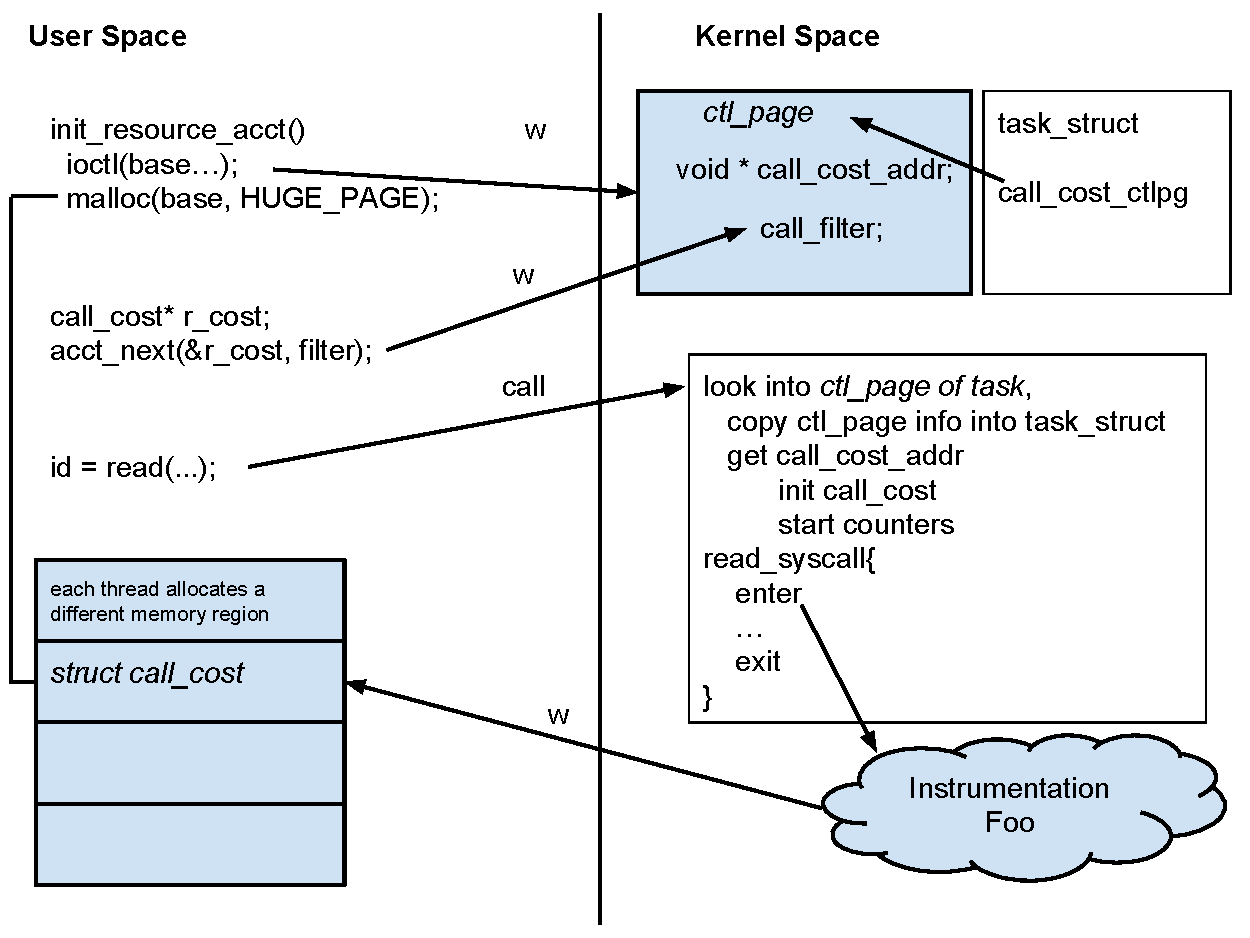
\includegraphics[width=\textwidth]{figures/system-design.pdf}
  \caption{An overview of library internals}
  \label{fig:sysDesign}
\end{figure}

\subsubsection{Library functions}
{\color{blue}\texttt{void init\_resource\_acct()}} initialises the library and must be called by each thread that intends to record any resource consumption. This triggers the following actions:
\begin{itemize}
\item memory allocation in user-space to hold \texttt{call\_cost} structures.
	\begin{itemize}
	\item The memory is allocated in user space by our library.
	\item We enable simple memory management on task switching (if the kernel switches the currently running process, it can look in the new \texttt{task\_struct} to find the resource accounting control page and the addresses of \texttt{call\_cost} structures for the newly executing process).
	\item The user does not need to do any memory mapping and can access the region normally. We use huge pages to reduce our impact on the TLB. The user-space will only read from this memory region.
	\item Having the memory managed by the user space library also means the application can decide when to reuse some \texttt{call\_cost} structures, without synchronizing with the kernel (as long as \texttt{async\_done} is true)
	\item A disadvantage of this is that accounting data stored for a process goes away when that process exits (normally or because of an error). We posit this is something that can be mitigated if needed (having a logging process with which each thread shares the memory containing accounting data; even if the process exits, the shared memory region will be kept as long as there is somebody referring to it). 
	\end{itemize} 
\item issue an ioctl to a char driver, setting up a 4K control page (\texttt{ctl\_page}) in the kernel and initializing our \texttt{task\_struct} field for the current task (\texttt{call\_cost\_ctlpg}) to point to that control page.
\item write the base address of the user-allocated memory region into the \texttt{ctl\_page}
\end{itemize}

{\color{blue}\texttt{int acct\_next(struct call\_cost**, u64 filter)}} indicates that the resource consumption of the next system call should be measured. The filter parameter is a logical \textsc{OR} between enum resource members (see section~\ref{evfilt} below).
\begin{itemize}
\item when called, the library looks for an available \texttt{call\_cost} entry in the memory region allocated for the current thread. It then writes the start address of this entry into the \texttt{ctl\_page}, together with the given filter. This data will be found and processed by the kernel on the next system call. 
\item because the programmer expresses interest above the glibc level (where system call are typically made), we might miss resource accounting for some system call: whenever one glibc function calls multiple system call the user can only account for the resource usage of the first. If on the contrary, glibc buffers some input (writes) and only calls a system call X once every n function calls, the user will end up sometimes measuring the cost of system call X and sometimes measuring the cost of whatever system call comes next. We consider such glibc calls “exotic” and we delay dealing with them to the second implementation pass.
\item on the second implementation pass we will also consider allowing the user to express interest in more than one system call (i.e measure resource utilization from now until a \texttt{stop\_accounting} function is called). 
\end{itemize}

{\color{red}\texttt{system call (rsrcfl library $\longleftrightarrow$ kernel)}} on any system call, on the kernel side we have to determine whether resource accounting needs to be done. We use system call interception in order to run our prologue code. This interception is achieved using the kernel's existing support for tracing. A sketch of what code we need to run before each system call is also displayed in Figure~\ref{fig:sysDesign}.
\begin{itemize}
\item We need to look into the current \texttt{task\_struct} and find the corresponding \texttt{ctl\_page} that contains both the memory address where we need to add accounting information and any filters the user might want. Those would be present if the user has set them up by calling \texttt{acct\_next}.
\item the kernel will initialize the given \texttt{call\_cost} structure as required
\item it will then start the required counters / snapshot desired values - in order to do the accounting (``Kernel accounting'' in Figure~\ref{fig:sysDesign}). More details on this are available in the section discussing the design of the required kernel extensions.
\end{itemize}

{\color{blue}\texttt{void cost\_callback\_async(struct call\_cost*, void (*cbk)(call\_cost*, void*), void*)}} registers a callback to be called when the asynchronous part of resource accounting has been completed. The second argument is the callback function pointer, which gets forwarded the actual \texttt{call\_cost} region containing the data and a \texttt{void*} context pointer.

{\color{blue}\texttt{int add\_to\_free\_stack(struct call\_cost *)}} indicates that the memory used by a struct \texttt{call\_cost} can be used to account for another system call. It is the responsibility of our library to decide how such regions should be reused (passed to the kernel for resource accounting) We anticipate this being called after the user has memcpy-ed the struct, performed some form of user-space aggregation or when the accounting data are no-longer required.

{\color{blue}\texttt{int add\_to\_free\_stack(struct call\_cost *[])}} same as above, but for multiple \texttt{call\_cost} structures

{\color{blue}\texttt{int stop\_async\_acct(struct call\_cost *)}} prevents further accounting of the async costs of the system call which is associated with the given \texttt{call\_cost}. This is basically a cancellation function. Any callbacks registered on the given \texttt{call\_cost} will still run at some point after the \texttt{stop\_async\_acct} returns.

\subsubsection{Data structures}

The user will mainly interact with \texttt{call\_cost} structures, which hold the resource accounting data for a particular system call. The interesting bits are the two accounting structures, one for synchronous costs and the other for asynchronous ones. The async costs should not be accessed if \texttt{async\_done} is false (the kernel is still updating the async costs).

\vspace{1em}
\begin{lstlisting}
/* Main structure for storing per-call resource consumption data
 */
struct call_cost {
  bool has_async;
  bool async_done;

  accounting sync;
  accounting async;
};
\end{lstlisting}

Each accounting structure contains a \texttt{cost\_bitmap} which is used to determine those kernel subsystems that were touched by the system call (and hence have associated resource accounting information). The \texttt{cost\_bitmap} contains a field which is a logical OR between resource enum members (the resource enum is shown below in section~\ref{evfilt}).

One design choice for the accounting struct was to make it fixed size (which in turn means \texttt{call\_cost} has a fixed size), for easy indexing within the allocated cost page. The first three components set in the \texttt{cost\_bitmap} field (starting from the LSB) are stored directly inside the struct (they will be cheaper to access for both the kernel and the user space). If any other components have accumulated cost, they will be stored in a dynamically allocated array which is pointed by ext.

\vspace{1em}
\begin{lstlisting}
struct accounting {
  cost_bitmap fields;   // logical OR of resource enum members

  acct_CPU cpu;         // aggregated CPU usage
  acct_Mem mem;         // aggregated Memory usage

  accounting_component[3] kunit_acct; // the first three subsystem costs
  int ext_no;
  accounting_component* ext;
};

union accounting_component {
  acct_Storage storage;
  acct_Net network;
  // ... etc
}

/* acct_*** data structures.
 */
struct acct_CPU {
  u64 cycles;
  u64 branch_mispredictions; //count
  u64 instructions; //count
};

struct acct_Mem {
  u64 alloc;
  u64 freed;
};

struct acct_Storage {
  acct_CPU cpu_costs;
  acct_Mem mem_costs;
  u64 avg_bandwidth;
  u64 io_wait;
  u64 seeks;
};

struct acct_Net {
  acct_CPU cpu_costs;
  acct_Mem mem_costs;
  tcp_info stats;
};
//.. others (one acct_*** structure per kernel subsystem - see the resource enum below)
\end{lstlisting}


\subsubsection{Event filtering}\label{evfilt}
A logical OR between resource enum members is used in the \texttt{acct\_next} call to let Resourceful know what it should track. A logical OR is also set by the kernel in the struct accounting \texttt{cost\_bitmap} when returning incurred costs to let the user know which parts of the kernel were touched (and hence have resource consumption data within a \texttt{call\_cost} structure)

\vspace{1em}
\begin{lstlisting}
/* The resource enum, together with the cost_bitmap structure, lets the end-user
 * quickly identify those kernel modules that were touched when a system call was made.
 * The corresponding acct_*** structures will be present in the accounting data
 * structure.
 *
 * A logical OR of resource members can also be explicitly passed by the user
 * when registering interest in system call resource accounting, as a filter.
 */
enum resource {
  SYS              = BIT(0),  // System functionality
  SYS_DEV          = BIT(1),  //  -- Device Model
  SYS_HW           = BIT(2),  //  -- Hardware Access
  SYS_IO           = BIT(3),  //  -- Device IO (USB, PCI, etc)

  PROC             = BIT(4),  // Processing functionality
  PROC_THR         = BIT(5),  //  -- Threading
  PROC_SYNC        = BIT(6),  //  -- Synchronization (locks)
  PROC_SCHED       = BIT(7),  //  -- Scheduler
  PROC_IRQ         = BIT(8),  //  -- Interrupts

  MEM              = BIT(9),  // Memory subsystem
  MEM_VIRT         = BIT(10), //  -- Virtual Memory
  MEM_MAP          = BIT(11), //  -- Memory Mapping
  MEM_PAGE         = BIT(12), //  -- Paging

  STORAGE          = BIT(13), // Storage subsystem
  STORAGE_VFS      = BIT(14), //  -- Virtual Filesystem
  STORAGE_CACHE    = BIT(15), //  -- Caching
  STORAGE_FS       = BIT(16), //  -- Filesystems
  STORAGE_HW       = BIT(17), //  -- Block Devices & Disk Controllers

  NET              = BIT(18), // Network subsystem
  NET_SOCK         = BIT(19), //  -- Sockets
  NET_PROTO        = BIT(20), //  -- Protocols
  NET_HW           = BIT(21), //  -- Hardware NIC Interface

  ALL              = ALL_BITS(21)
};

struct cost_bitmap {
  u32 primary; // logical OR between multiple resource elements
  
  #ifdef EXTENDED_ACCT_BITMAP // not used atm
  u64 ext;
  #endif
};
\end{lstlisting}

%  We provide a library that lets programmers access a struct that describes the cost of a system call. We require the program to specify that the next syscall should be accounted for, along with which components should be accounted for. After making the call, the user can access a struct that specifies the synchronous cost of making that syscall, per Linux subsystem. In particular, we do not perform function-level accounting, to reduce the overhead. Instead, we encourage developers to make use of existing tools, such as ftrace.
%
%  \subsection{Userspace API}
%  The resourceful API is exposed through a user-library.
%
%  Before performing a system call, a programmer can express that he wants the following syscall to be accounted for by calling the function \texttt{acct\_next}.
%  \texttt{acct\_next} takes two arguments: a pointer to a \texttt{struct call\_cost} and a filter. The \texttt{call\_cost} pointer is the address to which the kernel should write accounting information for the next system call to be made.
%  The filter is a bitmap representing which subsystems the user is interested in.
%
%  The \texttt{struct sys\_acct} contains an enum map that shows which subsystems were accessed by the system call followed by a section describing the costs for each subsystem touched. The programmer will read the touched subsystems, by reading the map, and then index into the relevant sections using offsets found from the map.
%
%
%  \subsection{Library API}
%  Our library has the following functions:
%  \begin{itemize}
%  \item \texttt{int call\_cost\_addr(struct call\_cost **, filter, n)} indicates that resourceful should track the next $n$ system calls to be made. The filter parameter indicates which subsystems it should be monitored through. The library is responsible for allocating memory for the accounting data to be stored in.\\
%design note: because the programmer expresses interest above the glibc level (where the system calls are typically made), we might miss resource accounting for some syscalls: whenever one glibc function calls multiple syscalls the user can only account for the resource usage of the first. If on the contrary, glibc buffers some input (writes) and only calls a syscall X once every n function calls, the user will end up sometimes measuring the cost of syscall $X$ and sometimes measuring the cost of whatever syscall comes next. We consider such glibc calls ``exotic'' and we delay dealing with them to the second implementation pass (it’s doable but requires more work).
%  \item \texttt{int add\_to\_free\_stack(struct call\_cost *)} marks that the memory used by a \texttt{struct call\_cost} can be used to account for another system call. We anticipate this being called after \texttt{memcpy}-ing the struct, or the data are no-longer required.
%  \item \texttt{int add\_to\_free\_stack(struct call\_cost *[])} is the same as the above, but for multiple \texttt{struct call\_cost}s. This has a lower overhead, as only one mode change is required.
%  \item \texttt{int stop\_async\_acct(struct call\_cost *)} prevents further accounting of the asynchronous costs in call\_cost.
%  \end{itemize}
%
%  This design puts responsibility for memory management on the library, rather than the kernel or the programmer. Naturally, programmers are not restricted to using our library.
%  \begin{description}
%  \item[On the first system call of each thread] the library will allocate:
%  \begin{enumerate}
%  \item One 4K page, known as the \texttt{ctl\_page}.  This is mapped RW in userspace, and is used to indiate to the kernel: whether to account for a system call; a pointer to where it should store accounting information; a bitmap of which subsystems we are interested in.
%  \item Some huge pages. We anticipate 4MB of space. This memory will be used as a buffer to store all accounting information. We use huge pages to reduce our load on the TLB. This must be mapped RO in  userspace.
%  \end{enumerate}
%  Moreover, the library issues an \texttt{ioctl} to a char driver, to inform the kernel of the start address of this buffer. The ioctl checks the protection bits on the page and will fail if mapped RW.
%  \item[On every system call we are accounting for]:
%  \begin{itemize}
%  \item  the library finds some free memory. A sensible implementation would be using a stack that stores pointers to slots in the buffer. This will cause reuse of the same addresses, thereby reducing the rate of trashing caches.
%  \item Writes the address that the accounting data should be stored in to the \texttt{ctl\_page}.
%  \item Returns with a pointer to the address that a \texttt{struct call\_cost} will be stored.
%  \end{itemize}
%  \end{description}
%
%  \subsection{Data structures}
%  The top-level data structure is \texttt{struct call\_cost}. This is a nested struct that contains the accounting cost of a system call, broken-down by subsystem. As most subsystems interact with CPU, memory, and at-most one other component (eg disk), we include a  bitmap  in struct call\_cost to indicate those components that are touched. We leverage this to allow us to store sparse data in the struct, thereby reducing our memory footprint.
%
%  \texttt{struct call\_costs} are expected to be stored in huge pages. We leave the management of where to store the struct within the huge pages to userspace. These huge pages must be mapped read-only by the userspace.
%
%  We also have a \texttt{struct ctl\_page}, which is a struct that exists for each thread and whose purpose it is to store the last address, and filters passed to \texttt{call\_cost\_addr}. Importantly we only have one value of this per thread, so each call to call\_cost\_addr will clobber the values written by the previous call. When a system call is made  we copy, in the kernel, the values written here so that we still have a pointer to the the \texttt{struct call\_cost} after we have executed \texttt{sysexit}, since we need to attribute asynchronous costs.

  \subsection{Kernel implementation}\label{kernelprimitives}

  In this section we describe our proposed use of \texttt{SystemTap} to allow fine-grained resource accounting.

  Figure~\ref{fig:sysDesign} shows the high-level flow of resourceful programs. Each process that requires fine-grained resource accounting issues a single \texttt{ioctl} to a char driver. The driver will allocate a 4K page, known as the \texttt{ctl\_page}, that is mapped R/W to the current process, and has its address stored in the relevant \texttt{task\_struct}. We expect the process to write the \emph{virtual} address of the location that the kernel should store accounting information into \texttt{ctl\_page.call\_cost\_addr}.

Throughout the kernel we use the value of \texttt{call\_cost\_addr} as the identifier of where to store the accounting data for ongoing operations.

  \subsubsection{Use of \texttt{SystemTap}}

We propose to use \texttt{SystemTap} to measure the resources used by system calls.
Our intended script will look to see if a new address has been written to the \texttt{ctl\_page}, and if so performs accounting.
 We add a probe to \texttt{sysenter} so it starts by checking the \texttt{ctl\_page.call\_cost\_addr} and \texttt{ctl\_page.filter} to see if the system call should be accounted for, and which metrics are desired.
Should these be set, we:
  \begin{enumerate}
  \item Copy the \texttt{\&call\_cost\_addr} and \texttt{filter} to a \texttt{SystemTap} variable.
  \item Check the validity of the values.
  \item Initialise \texttt{async\_ref\_cnt = 0}. We increase this counter on each asynchronous operation queued because of the current syscall; We decrement it when that asynchronous operation ends; We know the kernel has accounted for everything when the counter value goes back to 0 again.
  \end{enumerate}

  The system call will then enter its synchronous phase. We add probes to each boundary between kernel subsystem that:
  \begin{enumerate}
  \item Read all timers that we expect to be running, as specified by \texttt{filter}.
  \item Add the costs of these to the relevant subsection of the \texttt{struct call\_cost}. We can get the address of the \texttt{struct call\_cost} by deferencing \texttt{current->call\_cost\_addr} since, during the synchronous part of the system call, we can guarantee there will be no further system calls made by that task.
  \end{enumerate}

  We shall probe \texttt{sysexit}, with a function that will clobber \texttt{task\_struct.call\_cost\_addr} so as not to associate the next system call with the same \texttt{call\_cost\_addr} should it not be accounted for.

  After executing \texttt{sysexit} the kernel may have some latent work to do as part of the asynchronous operations in the system call. We intend to track the resources used by a syscall in both the synchronous, and asynchronous phases. As such we intend to modify the asynchronous mechanisms in Linux.  We note that Linux has a number of asynchronous mechanisms: \emph{kernel timers}, \emph{tasklets}, \emph{workqueues}, \emph{software interrupts}, and \emph{hardware interrupts}. To initialize each of these, the kernel calls a \texttt{\_\_init} function with a struct populated with relevant information. For instance to create a kernel timer, the \texttt{add\_timer} function\footnote{\texttt{kernel/timer.c}} is called with a \texttt{struct timer\_list}.

  As there are few functions on the interface to the kernel asynchronous mechanisms, each of which have a high number of call-sites.
  We propose to insert probes at functions that insert into \texttt{struct timer\_list} in \texttt{kernel/timer.c}, adding to it the \texttt{call\_cost\_addr} in the current context.

  We believe that tracking the \texttt{call\_cost\_addr} associated with asynchronous actions in the kernel is necessary, as without doing so:
  \begin{enumerate}
  \item It is unclear where we ought to allocate memory to store the accounting costs. We would therefore have to map more kernel memory, thereby likely making less-aggressive memory re-use, thereby incurring more caches misses, and TLB misses.
  \item We would have to track every metric for every asynchronous action in the kernel.
  \item It is no longer clear when all asynchronous actions have terminated for a given system call.
  \end{enumerate}
  
  A remaining discussion point is what to do when the cost of some asynchronous action should be split between multiple system calls (the case of flushing a buffer) In the first implementation, we propose keeping a list of \texttt{call\_cost\_addr} referring to the accounting structures of all the system calls involved. Those structures would be augmented to contain a scaling factor written during the synchronous part of the call (for example, the number of pending bytes that will be flushed asynchronously). Later, the user reading the \texttt{call\_cost} data will be able to scale the reported cost according to the fraction each call contributed to the cost.

  \subsubsection{Detecting subsystem boundaries}
  Resourceful accounts for resource consumption at a subsystem granularity.
  This requires us to define the functions that constitute a given subsystem and within these, the functions that act as an ingress point into it.
  Resourceful then uses these definitions to track which subsystem to credit resource consumption to.
  We employ a top-down approach when defining these systems by first observing the Linux kernel source directory structure, which provides a list of 5 subsystems. Within each of these there are then further layers of abstraction that need to be accounted for. These further layers are manually defined with the aid of the Linux kernel map.

  \begin{itemize}
      \item Storage (fs/)
      \begin{itemize}
	  \item Files and diectories
	  \item Virtual filesystem
	  \item Page cache, swap, network storage
	  \item Logical filesystem
	  \item Block devices
	  \item Disk controllers and drivers (drivers/)
      \end{itemize}
      \item Memory management (mm/)
      \begin{itemize}
	  \item Memory access
	  \item Virtual memory
	  \item Memory mapping, page cache, swap
	  \item Logical memory
	  \item Page allocator
	  \item Physical memory operations
      \end{itemize}
      \item Networking (net/)
      \begin{itemize}
	  \item Socket access
	  \item Protocol families
	  \item Networking storage
	  \item Protocols
	  \item Virtual network device
	  \item Nework device drivers (drivers/)
      \end{itemize}
      \item Processing (kernel/)
      \begin{itemize}
	  \item Processes
	  \item Threads
	  \item Synchronisation
	  \item Scheduler
	  \item Interrupt context
	  \item CPU specific (arch/)
      \end{itemize}
      \item System (kernel/)
      \begin{itemize}
	  \item System interfaces
	  \item Device model
	  \item System run
	  \item Generic HW access
	  \item Device access and bus drivers (drivers/)
      \end{itemize}
  \end{itemize}

  Note that some subsystems share functions for example the memory management subsystem implements part of the page cache along with the storage subsystem.
  Another observation is that due to the nature of abstraction, the lower the level the more machine specific, with many of the lowest levels either being implemented in device drivers (drivers/) or architecture specific code (arch/).


  In order to define the functions that constitute these subsystems we first use CTags to build a database of all functions along with the files they’re implemented in.
  Using this we are then able the tag each function with the top-level subsystem it belongs to (e.g. Networking || Processing).


  Resourceful accounts for resource consumption by checkpointing pre-defined resource counters at the entry and exit of each of these sub-systems.
  To enable this, the functions that act as entry points to these systems need to be identified, in order for them to be appropriately instrumented.
  These functions are identified by gathering function call traces of the target kernel using FTrace.
  The function calls in the resulting trace are then tagged with the top-level sub-system they belong to.
  The entry functions are then found by checking the boundaries between sub-systems, with the first function called in the sub-system being the entry.


  Further more specific sub-systems can be defined by annotating the original CTags list of symbols with the finer-grained system names. The same method as described above can be used to identify the sub-system entry functions.

  \subsubsection{Data structures required to store per-subsystem information}
  Resourceful relies on a list of per sub-system entry functions in order to instrument the kernel to achieve per sub-system resource accounting. The following data format is used to store these definitions of sub-systems:

  \begin{lstlisting}
  <function_name> - <top-level system> : {sub-system , ...} - <filename>
  \end{lstlisting}

  e.g.
  \begin{lstlisting}
  __get_free_pages - memory : page_allocator - mm/page_alloc.c
  \end{lstlisting}

  Each of the functions named in the list is instrumented by Resourceful as an entry point into the sub-system it is labeled with.
  
  \subsubsection{Existing primitives and kernel interfaces}\label{existingkernel}
  Those are elements already exposed by the kernel, and we will make use of them for (i) running additional code on particular function entry/exit points and (ii) getting the required resource consumption data.
  
  \begin{itemize}
  \item Kernel tracing
  	\begin{itemize}
  	\item ftrace kernel interface / mcount - requires root access
  	\item tracepoints - a few tools (perf \& SystemTap) already use these and they are fairly well adopted in the codebase
  	\end{itemize}
  \item Existing accounting mechanisms - when possible, we will use those instead of modifying the kernel data structures ourselves.
  	\begin{itemize}
  	\item perf\_events interface (software events use tracepoints, hardware events use the PMU)
  	\item taskstats \cite{taskstats} - provides a socket-based interface for accounting at task-level
  	\item latencytop \cite{latencytop}
  	\item getsockopt() - for TCP socket statistics
  	\item vmstat - Exported symbols allow loaded modules to gather information on the current VM status, including information such as page faults.
  	\end{itemize}
  \end{itemize}
  
    \subsubsection{Minimising overhead}
    We envisage Resourceful being an always-on component that exposes fine-grained accounting to allow a richer class of application. We therefore have an emphasis on low-performance overhead. Our design has the following features to reduce overhead:
    \begin{description}
    \item[Low impact on TLB.] We use huge pages to reduce the load on the TLB.
    We anticipate ~4MB of continuous memory being required per process. Using 4K pages, this might use one quarter of the TLB. By using huge pages we reduce this to two entries (assuming 2MB pages).
  
    \item[Minimal locking.] We aim to reduce concurrency mechanisms to limit our performance overhead. In particular, we store accounting data on a per-thread basis.
  
    \item[Minimal mode changes.] \texttt{sysenter}/\texttt{sysexit}  add a non-trivial overhead, especially when we want to debug the performance of single system calls. We therefore favour writing to shared-memory with atomic operations rather than making a syscall.
  
    \item[Zero-copy.] To improve performance we have avoided requiring the use of \texttt{memcpy}.
  
    \item[Shared memory strategy.] To reduce the number of mode switches, we make maximal use of shared memory. As a design choice we minimise pages being mapped RW to both userspace, and the kernel.
  
    \end{description}
  

  \section{Summary of work}

  We propose to write the following:
  \begin{description}[style=nextline]
  \item [Modify \texttt{task\_struct} to store \texttt{\&ctl\_page}, \texttt{\&call\_cost\_addr} and \texttt{filter}.]
    2 days
  \item[Write a char driver.] 2 days
    \begin{itemize}
    \item Basic setup to allow it to be \texttt{insmod}-ed.\\
      1/2 day
    \item Create a \texttt{ioctl} that will allocate a \texttt{ctl\_page}, map as R/O to current.\\
      1/2 day
    \item Write the address of the \texttt{ctl\_page} into \texttt{task\_struct}.\\
      1/2 day
    \end{itemize}
  \item[Provide a library that allows userspace programs to access synchronous accounting data.]
    2 days
    \begin{itemize}
      \item Create a header file that can be linked into an application.
        This should contain the \texttt{struct call\_cost} and library function declarations.\\
        1 day
      \item Implement \texttt{init\_resource\_acct}, which has to make the relevant ioctl.\\
        1/2 day
      \item Implement \texttt{call\_cost}, which has to copy its arguments into the correct memory address.\\
        1/2 day
    \end{itemize}
  \item[Interpose the \texttt{sysenter} routine to initiate accounting.]
\end{description}

\textsc{Milestone: have a working proof-of-concept that lets us measure the cost of performing the entirity of the synchronous phase of a system call.}

\begin{description}[style=nextline]
  \item[Provide a method of mapping the kernel into subsystems]
    days
    \begin{itemize}
      \item Find a benchmark that exercises a lot of the kernel.\\
        1 day
      \item Write a script that identifies subsystems from ftrace outputs.\\
        2 weeks
    \end{itemize}
  \item[Build the per-subsystem data structures]
    3 days
  \item[Build the snapshotting costs timeline]
    1 day
  \item[Modify all entry points so they take readings, and add them to the timeline]
    2 weeks
  \item[Modify exit points so they add their code back to the relevant \texttt{struct call\_cost}]
    2 days

\end{description}

\textsc{Milestone: be able to account for the synchronous part of a system call on a per-subsystem basis}

\begin{description}[style=nextline]
  \item[Extend our library to have a \texttt{cost\_callback\_async} method].
%    Implementation details tbc.
%    eg how does the library know when the async costs have finished.
%    We could look into how O_ASYNC works
    2 weeks
  \item[Modify the major asynchronous structs]
    2 weeks
  \item[Modify the entry and exit points to the asynchronous mechanisms to start accounting, and associate with the correct system call]
    2 weeks
\end{description}

\textsc{Milestone: be able to account for the asynchronous part of a system call, and have a callback once the asynchronous part has completed}

\subsection{Future work}
\begin{itemize}
\item Accounting for coallescing buffers.
\item Allow the user to express interest in multiple system calls being accounted for together
\item System-wide accounting
\item Exposing an interface in \texttt{/proc} to allow resourceful to be used without recompilation
\item Allow cancelling of accounting the asynchronous part of accounting for a system call
\end{itemize}

\subsection{SystemTap - implementation primitives}

\setlength\LTleft{-2.5cm}
\begin{longtable}{|p{9cm}|p{9cm}|}
\caption[]{The primitives required by the design together with SystemTap implementation solutions} \label{systemtap_impl} \\
\hline \multicolumn{1}{|c|}{\textbf{Required primitive}} & \multicolumn{1}{c|}{\textbf{SystemTap implementation}} \\ \hline
\endfirsthead

\multicolumn{2}{c}%
{{\bfseries \tablename\ \thetable{} -- continued from previous page}} \\
\hline \multicolumn{1}{|c|}{\textbf{Required primitive}} & \multicolumn{1}{c|}{\textbf{SystemTap implementation}} \\ \hline
\endhead

\hline \multicolumn{2}{|r|}{{Continued on next page}} \\ \hline
\endfoot

\hline \hline
\endlastfoot
\parbox{9cm}{transferring resource accounting data between kernel space and user space} & \parbox{9cm}{\vspace{2mm}- systemtap ring buffers (implicit), \\ - relayfs (per-cpu ring buffers that can be mmap-ed into user space)} \vspace{2mm}\\ \hline
\parbox{9cm}{per process/thread/syscall resource accounting selectors} & \parbox{9cm}{\vspace{2mm}- stap command line arguments -x (for tid, pid) or stap -c (for pid), probe filtering using the target() function. \\- per syscall invocation filtering is more involved (and requires cooperation from user space) } \vspace{2mm}\\ \hline
\parbox{9cm}{per-kernel-subsystem reporting of resource consumption} & \parbox{9cm}{\vspace{2mm}- from systemtap's perspective this is fully manual. in practice, we might be able to automatically or semi-automatically identify subsystem boundaries and generate the relevant bits of the systemtap script} \vspace{2mm}\\ \hline
\parbox{9cm}{measuring resource consumption} & \parbox{9cm}{\vspace{2mm}- start/stop timer probes on particular kernel functions (manual or semi-automatic determination of functions that need probing) } \vspace{2mm}\\ \hline
\parbox{9cm}{attributing async resource consumption to initial triggers (sync calls) } & \parbox{9cm}{\vspace{2mm}- data gathering probes: at sync function call, probe functions that write into shared data structures (buffers, queues, hash tables). get addresses of shared data structures \\- when measuring resource consumption of async-running task (kworker, swapper, sw/hw interrupts , kernel timers, workqueues, tasklets) determine which shared data structures (addresses) are touched and attribute resource consumption to the functions that created them \\- use systemtap associative arrays to store accounting data indexed per shared data structure address} \vspace{2mm}\\ \hline
\parbox{9cm}{accounting for coalescing buffers (the cost of those amortizes over multiple system calls)} & \parbox{9cm}{\vspace{2mm}- manual; a cost-assigning strategy has to be defined: initially, we'll go with proportionally splitting the costs amongst the system calls that placed items in such buffers} \vspace{2mm}\\ \hline
\parbox{9cm}{dynamically turning measurements on/off for subsystems of interest} & \parbox{9cm}{\vspace{2mm}- TBD; the slowest option would be to re-insmod the stap kernel module each time} \vspace{2mm}\\ \hline
\parbox{9cm}{determine actual time spent executing a call (for explaining perf. variations)} & \parbox{9cm}{\vspace{2mm}- probe all scheduler actions + interrupts} \vspace{2mm}\\ \hline
\parbox{9cm}{system-wide accounting} & \parbox{9cm}{\vspace{2mm}- implicit} \vspace{2mm}\\ \hline
\parbox{9cm}{canceling accounting of asynchronously-incurred costs} & \parbox{9cm}{\vspace{2mm}- user space cooperation required (relayfs?) \\ - remove addresses of shared data structures from the associative arrays} \vspace{2mm}\\ \hline
\parbox{9cm}{callback to user space after finishing asynchronous accounting (\texttt{cost\_callback\_async})} & \parbox{9cm}{\vspace{2mm}- user space cooperation required: relayfs + monitoring for changes (check if inotify is supported on relayfs)} \vspace{2mm}\\ \hline
\end{longtable}

  \begin{thebibliography}{1}

  \bibitem{kernelscale} \url{http://people.csail.mit.edu/nickolai/papers/boyd-wickizer-scaling.pdf}
  \bibitem{kernelmap} \url{http://www.makelinux.net/kernel_map/}
  \bibitem{taskstats} \url{https://www.kernel.org/doc/Documentation/accounting/taskstats.txt}
  \bibitem{latencytop} \url{http://lxr.free-electrons.com/source/kernel/latencytop.c}
  \end{thebibliography}


\end{document}
